\documentclass{article}

% Language setting
% Replace `english' with e.g. `spanish' to change the document language
\usepackage[english]{babel}
\usepackage{geometry}
\usepackage{algorithm}
\usepackage{algpseudocode}
\usepackage{svg}

\usepackage{lscape}

% Set page size and margins
% Replace `letterpaper' with `a4paper' for UK/EU standard size
 \geometry{
 a4paper,
 total={170mm,257mm},
 left=20mm,
 top=20mm,
 }
% Useful packages
\usepackage{amsmath}
\usepackage{graphicx}
\usepackage[colorlinks=true, allcolors=blue]{hyperref}

\title{Reasoning and Agents - Coursework 1}
\author{Finlay Ross-Davie}

\begin{document}
\maketitle

\section{Part A - Constraint Satisfaction Problems}

\subsection{A - Constraints}

Constraints:

$D = {1,2,3,4,5,6,7,8}$

\begin{equation}
GreaterThan(x,y)
    \begin{cases}
        if \: x > y \: then \: True \\
        otherwise \: False
    \end{cases}
\end{equation}

\begin{equation}
NotEqual(x,y)
    \begin{cases}
        if \: x \neq y \: then \: True \\
        otherwise \: False
    \end{cases}
\end{equation}

\begin{equation}
LessThanEqual(x,y)
    \begin{cases}
        if \: x \leq y \: then \: True \\
        otherwise \: False
    \end{cases}
\end{equation}


C = \{\

$NotEqual(a,b), \forall a, b \in destinations$ \newline
$GreaterThan(h_2,r_1)$ \newline
$GreaterThan(h_3, r_2)$ \newline
$GreaterThan(h_4, r_2)$ \newline
$GreaterThan(h_5, r_3)$ \newline
$GreaterThan(h_i,h_3), \forall i \in \{1,2,4,5\}$ \newline
$LessThanEqual(r_i,5), \forall i \in \{1,2,3\}$ \newline 

\}\

\subsection{B - Ternary Constraint}
Order 1 features a ternary constraint 

$(h_1, r_1, r_2) = (h_1 = max\{r_1, r_2\} + 1)$ \newline

$c = $\{\
$(R, r_1) = (R = r_1)$ \newline
$(R, r_2) = (R = max\{R, r_2\})$ \newline
$(h_1, R) = (h_1 = R+1)$ \newline
\}\

\subsection{C - Constraint graph}

\begin{figure}[ht]
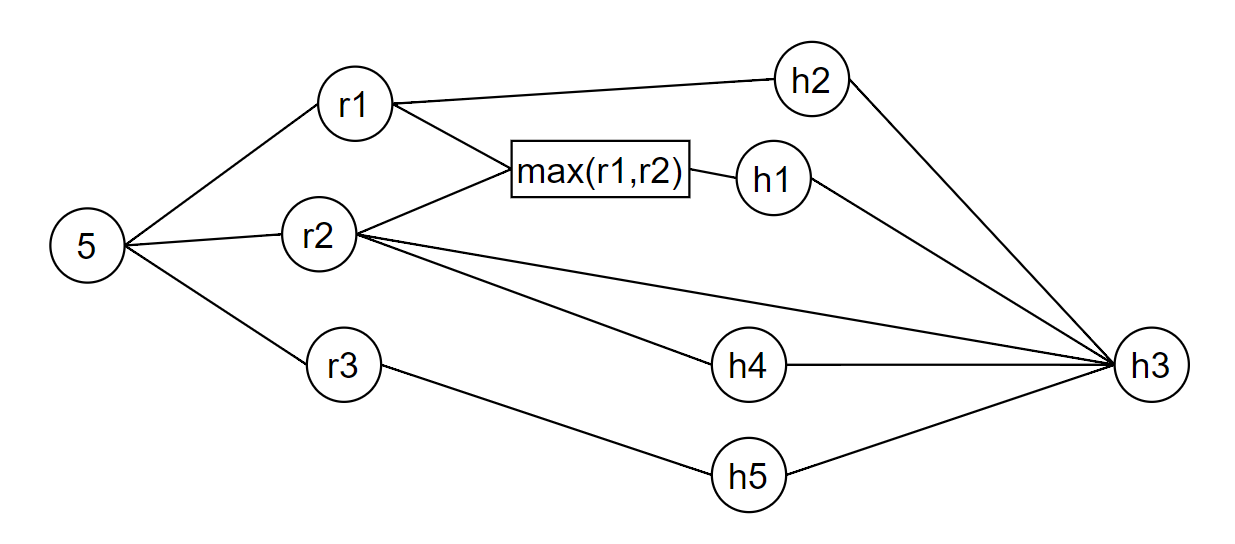
\includegraphics[width=8cm]{ConstraintGraph.png}
\centering
\end{figure}

\subsection{D - Backtracking search diagram}

 
\begin{landscape}

\begin{figure} {\centering \includesvg[width=28cm]{Constraint Graph-Backtracking Search Diagram.drawio.svg} }\end{figure}

\end{landscape}

\subsection{E - AC-3 diagram}

\begin{figure}[ht]
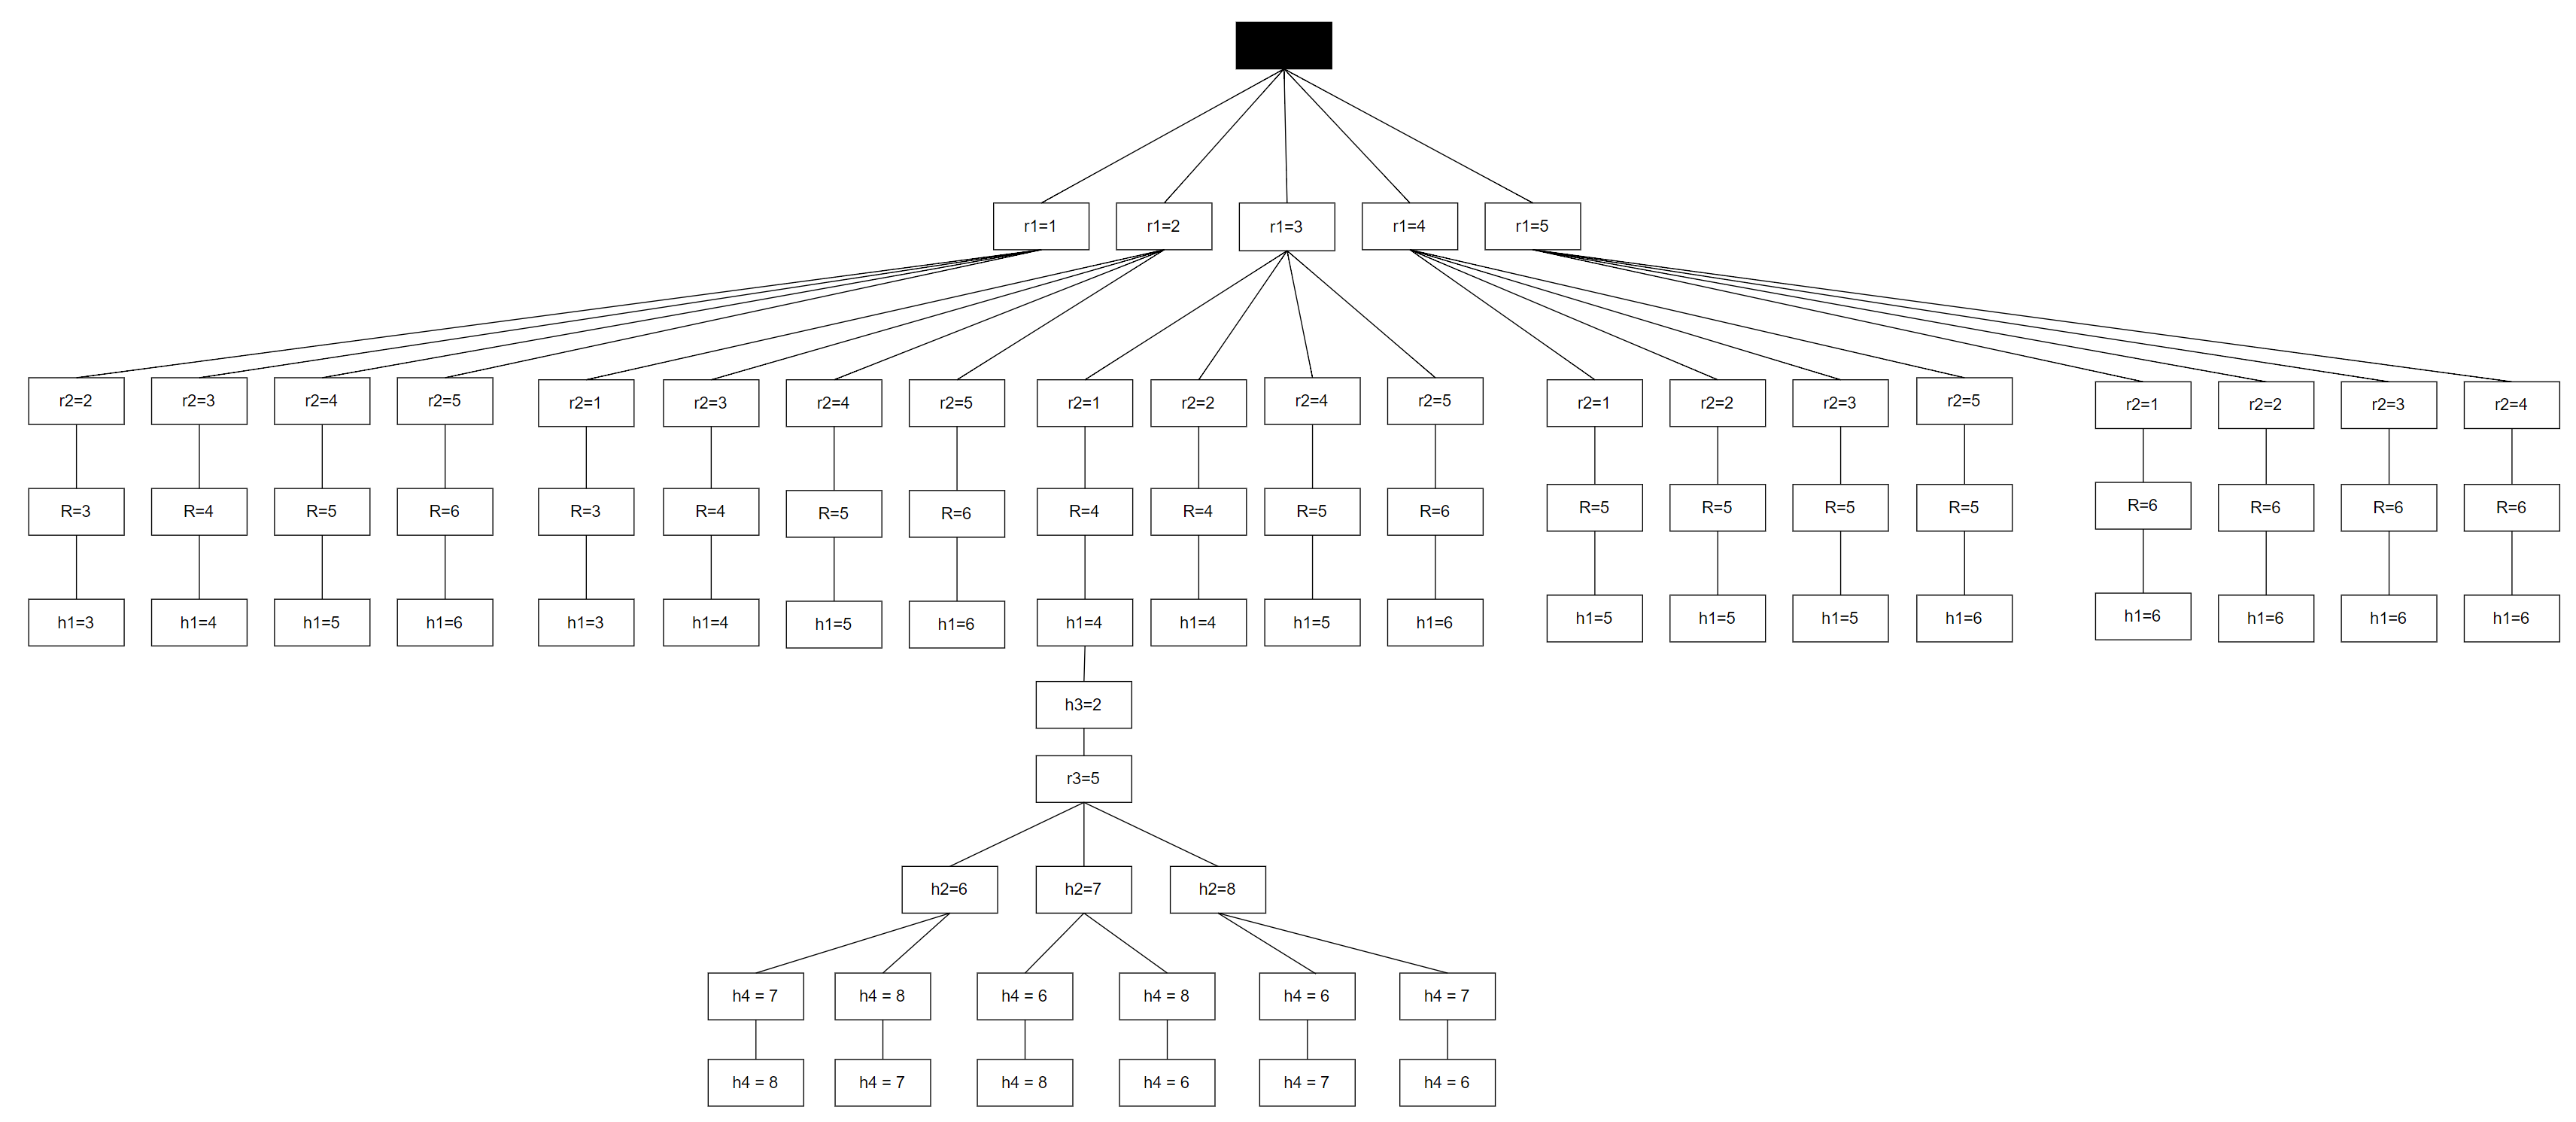
\includegraphics[width=18cm]{AC-3 Graph.png}
\centering
\end{figure}

\subsection{F - Pros and Cons}

AC-3 is far more efficient for this problem. For a similar problem in the future, I would choose AC-3 over backtracking search. 

\section{Part B - Search}

\subsection{A - Distance}

Manhattan distance would be an appropriate measure of distance, this is the sum of the horizontal and vertical distances which is applicable since drivers cannot move diagonally.

We can calculate it as:

For any two locations AB and CD where A and C represent the letter in the grid and B and D the number for each location, we can represent each letter with a number $0...16$, in ascending alphabetical order. $(x_1,y_1) = (A,B), (x_2,y_2) = (C,D)$.
E.g, the point C12 can be represented as (2,12)

The Manhattan distance can thus be represented as $$dist_M(l_1,l_2) = |x_1-x_2|+ |y_1-y_2|$$

\subsection{b - Driver heuristic}
$$ min\{dist_M(d_i, g)\}, \forall i \in \{1,2,3\}, \forall l \in goals$$

h1 driver: $$d_{h1} = min\{dist_M(d_i, r_1)\}, \forall i \in \{1,2,3\}$$
h2 driver: $$d_{h2} = min\{dist_M(d_i, r_2)\}, \forall i \in \{1,2,3\}$$
h3 driver: $$d_{h3} = min\{dist_M(d_i, r_3)\}, \forall i \in \{1,2,3\}$$

Using this heuristic we get 

h1 driver = H14
h2 driver = O1
h3 driver = P6

\subsection{c - A* Search}

\textbf{Driver 1} \newline
O1- r2 = N1 $\to$ M1 $\to $ M2 $\to$ M3 $\to$ M4 $\to$ L4 $\to$ K4 $\to$ J4 $\to$ I3 $\to$ I2 $\to$ I1 \newline
Nodes searched = N1,,M1, M2, O2 ,M3, N2, N3, M4, L4, K3, J4, K4, J4, I4, I3, I2 \newline
final frontier =  J5, I5, H4, H3, H2 \newline

path r2-h2 = I2 $\to$ I3 $\to$ I4 $\to$ I5 $\to$ I6 $\to$ J6 $\to$ J7 $\to$ J8 $\to$ J9 $\to$ J10 $\to$ I10 $\to$ H10 \newline
Nodes searched = I2, I3, I4, I5, I6, H2, H3, H4, H5, H6, G3, G4 G5, G6, F4,J4 ,J5,J6, J7, J8, J9, I10, H10, J11 \newline
final frontier = K4,F6,K6, L10,J11\newline

\textbf{Driver 2} \newline
P6 - r3 = P7 $\to$ P8 $\to$ P9 $\to$ O9 $\to$ O10 $\to$ O11 $\to$ O12 $\to$ O13 $\to$ O14 $\to$ O15 $\to$ O16 $\to$ P16 \newline
Nodes searched: P7, P8, P9, O6, O7, O8, O9, O10, O11, O12, O13, O14, O15, O16\newline
final frontier: N6, N7, N8, N9, N10, N11, N12, N13, N14, N15, N16 \newline


path r3 - h3:

P16 - N3 = P15 $\to$ P14 $\to$ N14 $\to$ N13 $\to$ N12 $\to$ N11 $\to$ N10 $\to$ N9 $\to$ N8 $\to$ N7 $\to$ N6 $\to$ M6 $\to$ L6 $\to$ K6 $\to$ J6 $\to$ J5 $\to$ J4 $\to$ K4 $\to$ L4 $\to$ M4 $\to$ M3 $\to$ N3

Nodes searched: P15, O16, O15, N16, N15, O15, N14, O14, M15, N13, O13, M14, N12, O12, M13, N11, O11, M13, N10, O10,M12, N9, O9, M11, N8, O8, M10, N7, O7, M9, N6, O6, M8, P9, P8, P7, P6, M7, M6, L15, K15, J15, J14, J13, J12, J11, J10, K10, L10, J9, J8, J6, J5, J4, K4, L4, M4, M3 \newline

final frontier: J16, I4, I5, I6, I10, M2

\textbf{Driver 3} \newline
path start h14 - r1: G14 $\to$ F14 $\to$ E14 $\to$ D14 $\to$ C14 $\to$ B14 $\to$ A14
Nodes searched: G14, F14, E14, D14, C14, B14, A14
Final Frontier: G13, F13, E13, E15,D13, C13, B13, A13


path start r1 - h1: B14 $\to$ B13 $\to$ B12 $\to$ B11 $\to$ B10 $\to$ C10 $\to$ C9 $\to$ D9 $\to$ E9 $\to$ E8 $\to$ E7 $\to$ E6 $\to$ E5 $\to$ E4 $\to$ E3 $\to$ E2 $\to$ E1 \newline

Nodes Searched: A13, B14, B13, C14, B12, C13, B11, C12, D14, B10, C11, B9,,C9 B8,C8  C10, E14, E14, D11, E13, D10, E12, D9, E11, E10, E9, E8,E7,E6, E5, E4, E3, E2, E1 

Final Frontier: A12, A11, A10, A9, E15, F14, F13, F12, F11, F10, F4, D6, D5, D4, D3\newline



\subsection{d - Puesdocode Algorithm}

\begin{algorithm}
\begin{algorithmic}

\Procedure{FIND-SHORTEST-ROUTE}{$problem$}

\Comment{FIND-SHORTEST-ROUTE returns the shortest route as an array of desinations with $shortestRoute[0]$ representing the start and $shortestRoute[5]$ the final desintiation}

\Comment{The procedure takes the problem argument which contains the initial driver location, grid, and positions of destinations}

\Comment{The procedure makes use of the FIND-SHORTEST-ROUTE procedure in Fig 3.26 in Russell \&\ Norvig 3rd Ed and makes use of the Manhattan heuristic} \newline

\State Set routes to the permutations of destinations \Comment{Stored as a list of route lists}

\State Set minDistance to $\infty$
\State Set shortestRoute to $[]$ \newline

\For{each route in the routes list} \newline

    \State set exploredDestinations to []

    \State set currentLength to zero \newline

    \For{each destination in route}

        \If{destination is a house} \Comment{Enforcing restruant before house constraint}

            \If{restaurant corresponding to the destination is not in exploredDestinations} 
                \State break the current iteration of the outer loop and move to next route
            \EndIf

        \EndIf
    
        \State Set currentDistance to the length of \textit{RECURSIVE-BEST-FIRST-SEARCH($subProblem$)} \Comment{Where the \textit{subProblem} is the general problem with start defined as the current destination and the next destination in the list as the goal} \newline

        \State Compute currentLength as currentLength + currentDistance 

        
        \If{currentLength $>$ minDistance}
            \State break the current iteration of the outer loop and move to next route\newline
        \EndIf       
        
    \EndFor


    \If{currentLength $<$ minDistance}
        \State set minDistance to currentLength
        \State set shortestRoute to route     
    \EndIf

    \State Append destination to exploredDestinatons \newline    
\EndFor

\State return shortestRoute
    
\EndProcedure \newline

\end{algorithmic}
\end{algorithm}

\subsection{e - Assigning Drivers}

Using the Manhattan distance heuristic, we could assign each driver to its closest restaurant and from the restaurant deliver to the corresponding house. We can repeat this process simply changing the comparison point to the location of the house in the last order, each time finding the shortest Manhattan distance to all restaurants. \newline

1. Initial Setup: Each driver starts with the order associated with their closest respective restaurant found by applying the Manhattan Heuristic to all points in the grid. \newline

2. Assignment Loop: While there are still destinations remaining:

2.1. For each Driver: Determine the shortest Manhattan distance between the current location (house belonging to last order in the list) of each driver and each restaurant in the grid. If another driver has the same closest restaurant, assign the restaurant to the driver with the lower Manhattan value and find the next closest restaurant for the driver with the higher Manhattan value, repeat this process until each driver as its own distinct restaurant for the current iteration. 

2.2. Select Next Destination: Append the order associated with the restaurant that has the shortest Manhattan distance to the drivers list and remove the destinations (house and restaurant of the order) from the list of remaining destinations

This solution is not globally optimal but does provide an approach to \textbf{reduce} the total distance in a large number of scenarios

\subsection{f - Improvements}

During A* Search, when two nodes have the same value generated by the evaluation function, we should choose to expand one and only backtrack to the other if the expansion of the chosen node leads to a repeated state or empty frontier. 

\subsection{g - Improvement Puesdocode}

\begin{algorithm}
\begin{algorithmic}

\Procedure{MODIFIED-STAR-SEARCH}{$graph, startNode, goalNode$}

\For{node in graph}
    \State Set node.score to infinity 
    \State Set node.heuristicScore to infinity
    \State Set node.visited to false
    \State Set node.ignore to false
\EndFor

\State Set startNode.score to 0
\State Set startNode.heuristicScore to 0 \newline


\While{true}
    \State Set currentNode to nodeWithLowestScore
    \State Set currentNode.visited to true \newline


    \For{neighbour in neighbours of currentNode}
        \If{neighbour.visited is false and neighbour.ignore is false}
            \State Set newScore to currentNode.score + 1
            \If{newScore is less than neighbour.score}
            
                \State Set neighbour.score to newScore
                \State Set neighbour.heuristicScore to newScore + evaluationFunction(neighbour, goalNode)
                \State Set neighbour.routeToNode to currentNode 
                
            \EndIf      
        \EndIf
    \EndFor \newline

    \If{currentNode is equal to targetNode}
        \State \textbf{return} buildPath(targetNode)
    \EndIf \newline

    \If{nodeWithLowestScore(graph).score is equal to infinity}
    \State Set lowestIgnore to null
        \For{node in graph}
            \If{node has not been visited and node.heuristicScore < result.heuristicScore and node.ignore is true}
                \State Set lowestIgnore to node
            \EndIf        
         \EndFor 
        \State Set lowestIgnore.ignore to false \newline

        \If{lowestIgnore is null}
            \textbf{return} no path has been found
        \EndIf \newline
    
        
    \EndIf \newline

\EndWhile
\EndProcedure \newline

\Procedure{nodeWithLowestScore}{$graph$}
    \For{node in graph}
        \If{node has not been visited and node.heuristicScore $<$ result.heuristicScore and node.ignore is false}
            \State Set result to node
        \EndIf        
    \EndFor \newline

    \For{node in graph}
        \If{node has not been visited and node is not result and node.heuristicScore = result.heuristicScore}
            \State set node.ignore to true
        \EndIf
    \EndFor 

\EndProcedure


\end{algorithmic}
\end{algorithm}


\end{document}